\documentclass[winfonts,UTF8,a4paper]{ctexart}
%%package
\usepackage[lined,boxruled,commentsnumbered]{algorithm2e}
\usepackage{amsfonts}
\usepackage[figurewithin=section]{caption}
\usepackage{color}
\usepackage{fancyhdr}
\usepackage{floatrow}
\usepackage[text={160mm,247mm},left=30mm,right=20mm,includeheadfoot,vmarginratio=1:1]{geometry}
\usepackage{graphicx}
\usepackage{listings}
\usepackage[numbers,sort&compress]{natbib}
\usepackage{setspace}
\usepackage{tabularx}
\graphicspath{{graph/}}
%%Define colors
\definecolor{keywordcolor}{rgb}{0.8,0.1,0.5}
\definecolor{webgreen}{rgb}{0,0.5,0}
\definecolor{shadowcolor}{RGB}{190,190,190}
%% listings settings
\renewcommand{\lstlistingname}{代码}
\lstset{
basicstyle=\rmfamily\footnotesize,
keywordstyle=\color{keywordcolor}\bfseries, %\underbar,
commentstyle=\color{blue} \textit,
stringstyle=\ttfamily,
showstringspaces=false,
frame=shadowbox,
rulesepcolor=\color{shadowcolor},%\color{red!20!green!20!blue!20},
xleftmargin=2em,
xrightmargin=2em,
aboveskip=1em
}
%重设Code环境
\lstnewenvironment{code}[1][]%
{
   \noindent
   \minipage{\linewidth}
   \vspace{0.5\baselineskip}
   \lstset{basicstyle=\rmfamily\footnotesize,
           keywordstyle=\color{keywordcolor}\bfseries,
           commentstyle=\color{blue} \textit,
           stringstyle=\ttfamily,
           showstringspaces=false,
           frame=shadowbox,
           rulesepcolor=\color{shadowcolor},
           xleftmargin=2em,
           xrightmargin=2em,
           aboveskip=1em,#1}
}{\endminipage}
%%参数设置
\onehalfspacing %%1.5倍行距
\renewcommand{\footnotesize}{\zihao{5}}%%设置脚注字号
\floatsetup[table]{capposition=top}%%表格标题在表格上方
%页眉,页脚
\pagestyle{fancy}
\fancyhf{}
\fancyhead[C]{\zihao{-5} 暨南大学本科课程论文}
%重设节标题
\CTEXsetup[format={\zihao{-2}\songti\bf\flushleft}]{section}
\CTEXsetup[format+={\zihao{4}\songti}]{subsection}
\CTEXsetup[format+={\zihao{4}\songti}]{subsubsection}
%重设图片、表格标号
\makeatletter
    \renewcommand{\thefigure}{\ifnum \c@section>\z@ \thesection-\fi \@arabic\c@figure}
    \renewcommand{\thetable}{\ifnum \c@section>\z@ \thesection-\fi \@arabic\c@table}
\makeatother
%重设目录格式
%\usepackage{titletoc}
%\titlecontents{section}[2em]{\vspace{3mm}\zihao{4}\songti\bf}{\contentslabel{1.7em}}%
%    {}{\bf\titlerule*[0.5pc]{$\cdot$}\zihao{4}\contentspage}
%\titlecontents{subsection}[2.5em]{\zihao{-4}\songti}{\thecontentslabel}%
%    {}{\titlerule*[0.5pc]{$\cdot$}\zihao{-4}\contentspage}
%\titlecontents{subsubsection}[2.5em]{\zihao{5}\songti}{\thecontentslabel}%
%    {}{\titlerule*[0.5pc]{$\cdot$}\zihao{5}\contentspage}

\begin{document}
  %%--------------- 前言 ----------------- %%
    \begin{center}
  \zihao{2}\textbf{\kaishu 诚 ~~ 信 ~~ 声 ~~ 明}
\end{center}\par
\vspace{10mm}
\zihao{-3}
\kaishu
我声明,所呈交的课程论文是本人在老师指导下进行的研究工作及取得的研究成果。据我查证,除了文中特别加以标注和致谢的地方外,论文中不包含其他人已经发表或撰写过的研究成果,也不包含为获得其他教育机构的学位或证书而使用过的材料。我承诺,论文中的所有内容均真实、可信。\\[45mm]
课程论文作者签名:\hspace{30mm}签名日期:\qquad 年\quad 月\quad 日
\newpage

    \songti
\begin{center}
  \zihao{-2}\textbf{可视化的Java多线程程序错误定位工具}
\end{center}
\vspace{10mm}
\zihao{4}\textbf{摘要}\par
随着多核CPU的出现,多线程程序在软件开发领域得到广泛的应用。与此同时,多线程程序当中的并发错误也给软件开发者带来的很多困难。2009年,Sangmin Park等人提出了名为Falcon的新方法用来进行多线程程序中并发错误的错误定位。该方法可以按照可疑度的大小报告程序中的数据访问模式。但是,Falcon纯文本的展示方式仍然不便于程序员快速定位错误。所以在本篇论文中,作者首先介绍Falcon的实现原理,然后以Falcon为基础,开发一个可视化的Java多线程程序错误定位工具。
\\[10mm]
\textbf{关键词:错误定位;软件调试;Java;多线程}
\newpage

%English Abstract
\begin{center}
  \zihao{-2}\textbf{Visual Fault Localization Tool for Java Multi-threaded Program}
\end{center}
\vspace{10mm}
\zihao{4}\textbf{Abstract}\par
With the widespread deployment of multi-core processors, multi-thread programming becomes popular in software industry. Meanwhile, concurrent faults in multi-threaded programs cause troubles to software developers. In 2009, Sangmin Park \textit{et al.} presented a new dynamic fault-localization technique to locate concurrent faults in multi-thread programs. It can report data access patterns with suspiciousness scores. However, the results are presented in plain text format which are still hard to read and analyze for programmers. This paper introduces Falcon's algorithm and then implements Falcon approach with a visualization tool.
\\[10mm]
\textbf{Keywords:Fault localization; Software debuging; Java; Multi-threaded}


    \tableofcontents
 \thispagestyle{empty}
 \newpage

%%----------------- 正文 ----------------- %%

%重设页眉,页脚
\pagestyle{fancy}
\fancyhf{}
\fancyhead[C]{\zihao{-5} 可视化的Java多线程程序错误定位工具}
\fancyfoot[R]{\thepage}
%重设页码
\setcounter{page}{1}
\pagenumbering{arabic}
    \section{课题背景}
近年来,随着多核处理器的出现和迅速发展,并行计算、多线程程序逐渐在软件开发领域得到了广泛的使用。与此同时,并行计算的广泛使用也给软件测试提出了新的挑战。
\subsection{程序的并发错误}
因为并行程序本身的特点和缺乏有效的并行程序设计方法与工具,使得正确编写并行程序,调试和优化并行程序都很困难。一方面,编写并行程序比编写串行程序更加困难。除了串行程序常见的错误\footnote{在本篇论文中,漏洞、缺陷、错误可以互换地使用。}之外,并行程序还有诸如死锁、数据争用等独有的错误。所以一段并行程序中存在错误的可能性更大。另一方面,测试并行程序比测试串行程序更加困难。这是因为:第一,并行程序的运行结果具有不确定性,难以重现错误;第二,程序的运行结果牵涉到多线程操作,使得错误不易定位\cite{mcdowell1989debugging}。\par
微软公司在2007年发布的针对684名员工的调查报告显示66\%的受访者需要经常处理并发程序中的问题(包括测试、调试、修复)。超过72\% 的受访者认为重现并行程序中的错误困难或非常困难,63.4\%的受访者需要花费数天才能解决并行程序中的错误。在微软公司的调查报告中,受访者把更好的错误定位工具放在了他们需求的首位\cite{godefroid2008concurrency}。由此可见,在软件开发的过程中,并发程序中的错误制约了软件开发效率。软件开发领域需要一款能够准确地在并发程序中进行错误定位的工具。
\subsection{Java并发程序的错误定位技术}
在软件调试过程中,错误定位是识别程序中错误准确位置的活动。软件调试是软件开发过程中最费时费力的活动,而错误定位又是调试过程中最费时费力的活动。所以,软件开发领域中需要错误定位技术来指导程序员找到程序中的错误\cite{wong2009survey}。\par
为了解决Java并发程序错误定位这个问题,一些学者经过不断的努力,提出了多种方法。Ronsee等人提出了一种方法可以用来检测数据争用,并且可以记录和重复并发程序\cite{RecPlay}。Shan Lu等人尝试通过检识别非顺序的线程交错来检测原子性破坏(AVIO)\cite{AVIO}。
\subsection{Java程序的并发错误}
\subsubsection{标识说明}
在具体描述这两种数据访问模式之前,首先约定本篇论文中关于不同线程对共享变量读写的表述方式。本文使用$b_{t,S}$来表示一个线程访问了一个共享变量。其中$b$是访问的类型,分为读($R$)或者写($W$)两种;$t$表示操作变量的线程,通常用线程号(一个整数)进行表示;$S$ 表示含有被访问的共享变量的语句。例如,$R_{1,S2}$表示线程1在语句$S2$中对一个共享变量进行了读操作。有的时候可以通过上下文得出含有共享变量的被访问语句,所以为了简化描述,后文中也会在不影响理解的情况下将$R_{1,S2}$简写为$R_1$。
\subsubsection{错误类型的划分}
如果想要定位并发程序中的错误,首先要能够发现并发错误出现的规律和找到并发错误的方法。近年来,学者们尝试建立了一些有错误倾向的数据访问模式(data access pattern),如果在并发程序运行的过程中,不同线程访问共享数据的方式符合这些数据访问模式,就有出现并发错误的可能性。这些数据访问模式包括两种:顺序破坏(order violation)和原子性破坏(atomicity violation)。\\
\textbf{顺序破坏}\par
顺序破坏就是访问一个共享变量的两个线程(其中一个线程进行写操作)因为访问顺序交错导致读、写错误的数据。顺序破坏一共有三种形式,如表\ref{tab:ConflictingInterleavingPatterns}所示。
  \begin{table}[!ht]
    \centering
    \zihao{4}
    \caption{顺序破坏模式}\label{tab:ConflictingInterleavingPatterns}
    \begin{tabular}{|c|c|c|}
      \hline
        & 线程读写 & 描述 \\\hline
      1 & $R_1-W_2$ & 写入意外的数值 \\\hline
      2 & $W_1-R_2$ & 读出意外的数值 \\\hline
      3 & $W_1-W_2$ & 线程1写入的数值丢失 \\
      \hline
    \end{tabular}
  \end{table}\\
\textbf{原子性破坏}\par
一个原子操作是指不会被线程调度机制打断的操作;这种操作一旦开始,就一直运行倒结束,中间不会被其它线程打断,否则就可能会产生错误。这种不可被打断的特性被称作原子性。原子性破坏就破坏了原子操作的原子性,即一个线程操作共享变量的过程中,另外一个线程操作被错误的插入。原子性破坏一共有5种形式,如表\ref{tab:UnSeInterleavingPatterns}所示。
 \begin{table}[!ht]
    \centering
    \zihao{4}
    \caption{原子性破坏模式}\label{tab:UnSeInterleavingPatterns}
    \begin{tabular}{|c|c|c|}
      \hline
        & 线程读写 & 描述 \\\hline
      1 & $R_1-W_2-R_1$ & 不可重复读 \\\hline
      2 & $W_1-W_2-R_1$ & 线程1数据被线程2意外修改 \\\hline
      3 & $W_1-R_2-W_1$ & 线程2读入错误数据 \\\hline
      4 & $R_1-W_2-W_1$ & 丢失修改 \\\hline
      5 & $W_1-W_2-W_1$ & 丢失修改 \\
      \hline
    \end{tabular}
  \end{table}
\subsection{Falcon方法}
2009年,乔治亚理工学院(Georgia Institute of Technology)的Sangmin Park等人提出了一个名为Falcon(Fault Localization in Concurrent Programs)的新方法。Falcon可以定位多线程并发程序中错误的数据访问模式,并且可以根据被测程序的通过、失效数给出每个数据访问模式的可疑度,从而便于用户快速地定位错误\cite{park2010falcon}。用户可以根据Falcon得到的可疑度,找出最有可能存在错误的数据访问模式,然后根据数据访问模式的信息可以定位到该错误所在的行号和变量。\par
Falcon算法通过两个步骤来识别程序中的多线程错误。第一步,需要实时地监测程序不同线程对共享变量的访问,并识别、记录下程序运行过程中出现的访问模式。第二步,需要对第一步得到的数据进行统计和分析,结合测试用例的执行结果(通过或失效),得到每一个访问模式的可疑度,并按照可疑度的大小从高到低排序。\par
和以往的错误定位工具的工作原理相比,Falcon有两点不同:
\begin{enumerate}
  \item Falcon多次执行同一个测试用例,而不是执行多个测试用例;
  \item Falcon并不追求覆盖更多的代码,而是尝试记录数据访问模式。
\end{enumerate}
\subsubsection{实例}\label{sec:Example}
在具体介绍Falcon算法之前,本节先给出一段伪代码程序。然后本文将在\ref{sec:recongnizePattern}和\ref{sec:rankPattern}两节再使用这个具体的实例来演示Falcon 算法,依次介绍Falcon的两个主要步骤。\par
下面的伪代码描述的是一段包含有三个线程,两个共享变量的程序。
\begin{lstlisting}[language={[AspectJ]Java}, label=lst:code, caption=示例伪代码]
      x=0; y=0;
      Thread1
      1: if(x==0) x=1;
      2: if(y==0) y=1;
      3: if(x==2 and y==2) assert(false);
      Thread2
      4: if(x==1) x=2;
      5: if(y==1) y=2;
      Thread3
      6: if(x==1) x=3;
      7: if(y==1) y=3;
\end{lstlisting}\par
由于多线程程序的运行结果并不确定,本文假设4种可能出现的执行语句序列及相应的对变量x和变量y的访问序列,如表格
\ref{tab:exeResult} 所示。
\begin{table}[!ht]
    \centering
    \resizebox{\textwidth}{!}{
    \caption{4种可能的运行结果}\label{tab:exeResult}
    \begin{tabular}{|c|c|c|c|}
      \hline
        & 执行语句序列 & 对x的访问序列 & 对y的访问序列\\\hline
      1 & 1-6-4-2-7-5-3 & $R_{1,1}-W_{1,1}-R_{3,6}-W_{3,6}-R_{2,4}-R_{1,3}$ & $R_{1,2}-W_{1,2}-R_{3,7}-W_{3,7}-R_{2,5}-R_{1,3}$ \\\hline
      2 & 1-6-4-2-5-7-3 & $R_{1,1}-W_{1,1}-R_{3,6}-W_{3,6}-R_{2,4}-R_{1,3}$ & $R_{1,2}-W_{1,2}-R_{2,5}-W_{2,5}-R_{3,7}-R_{1,3}$ \\\hline
      3 & 1-4-6-2-7-5-3 & $R_{1,1}-W_{1,1}-R_{2,4}-W_{2,4}-R_{3,6}-R_{1,3}$ & $R_{1,2}-W_{1,2}-R_{3,7}-W_{3,7}-R_{2,5}-R_{1,3}$ \\\hline
      4 & 1-4-6-2-5-7-3 & $R_{1,1}-W_{1,1}-R_{2,4}-W_{2,4}-R_{3,6}-R_{1,3}$ & $R_{1,2}-W_{1,2}-R_{2,5}-W_{2,5}-R_{3,7}-R_{1,3}$ \\
      \hline
    \end{tabular}}
\end{table}
\subsubsection{访问模式识别}\label{sec:recongnizePattern}
Falcon的第一步就是要获取和识别程序执行过程中出现的数据访问模式,具体的算法如算法\ref{algo:GP}所示。当被测程序运行的时候,Falcon使用一个固定大小的滑动窗口来识别模式,因而需要解决滑动窗口的更新和实时模式识别这两个问题。
\renewcommand{\algorithmcfname}{算法}
  \begin{algorithm}
    \SetAlgoCaptionLayout{centerline}%标题居中
    \caption{GatherPatterns\label{algo:GP}}
    \DontPrintSemicolon
    \SetKwFunction{createWindow}{createWindow}
    \SetKwFunction{registerWindow}{registerWindow}
    \SetKwFunction{getWindow}{getWindow}
    \SetKwFunction{getPatterns}{getPatterns}
    \SetKwFunction{slideWindow}{slideWindow}
    \SetKwInOut{Input}{输入}
    \SetKwInOut{Output}{输出}
    \Input{$m$:shared memory location\\
    $b$:memory access type\\
    $t$:thread ID\\
    $s$:meomory access location\\
    $P_t$:current set of patterns(initially null)}
    \Output{$P_t$:updated set of patterns}
    \BlankLine
    \eIf{$m$ does not yet have any window}{
      w$\leftarrow$\createWindow{}\\
      $w$.insert($b,t,s$)\\
      \registerWindow{$w,m$}
    }
    {
      w$\leftarrow$\getWindow{$m$}\\
      ($b_2,t_2,s_2$)$\leftarrow w$.getLastAccess()\\
      \eIf{$t=t_2$}{$w$.update($b,s$)}{
        \If{$w$ is full}{
        $P_t\leftarrow$\getPatterns{$w$}\\
        $w\leftarrow$\slideWindow{$w$}
        }
        $w$.insert($b,t,s$)
      }
    }
    \Return{$P_t$}
  \end{algorithm}\\
\textbf{滑动窗口的更新}\par
初始时,窗口是空的,因此,窗口将会存入第一个线程访问变量的记录。如果新出现的记录和之前的记录属于不同的线程(即一个线程逃逸访问),新记录则被存入在窗口的空位中。然后继续读入记录,如果新出现的记录和之前的记录属于同一个线程(即一个线程本地访问),新的记录则替换原有的记录。需要注意的是:因为线程的写操作更容易产生错误(在顺序破坏和原子性破坏中都至少有一个写操作),所以若新的记录是读操作,则不替换原有写操作的记录。\par
\begin{figure}[!ht]
  \centering
  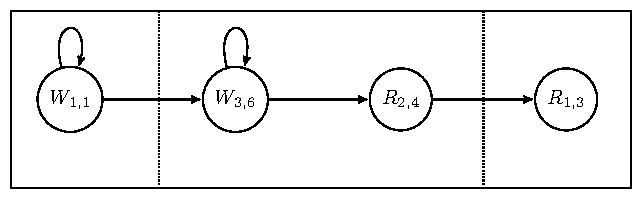
\includegraphics[width=.8\textwidth]{SlidingWindow_x.pdf}
  \caption{滑动窗口示例}\label{pic:slidingWindow}
\end{figure}
对于\ref{sec:Example}给出的实例,取表\ref{tab:exeResult}中第一个运行情况进行讨论,对变量x的访问序列是$R_{1,1}-W_{1,1}-R_{3,6}-W_{3,6}-R_{2,4}-R_{1,3}$。滑动窗口如图\ref{pic:slidingWindow} 所示。
开始是线程1连续两次对变量操作$R_{1,1}-W_{1,1}$。滑动窗口首先读入线程1的读操作$R_{1}$,接着又读入了线程1的写操作$W_{1}$,因为两次访问都是同一个线程,所以滑动窗口向前滑动,只记录$W_1$。同理,窗口内又读入了$W_3$和$R_2$。当滑动窗口已满的时候,则移除最早的记录。对于图所示的滑动窗口,窗口大小是3,当读入线程2的操作$R_{2,4}$时,窗口已满,则窗口滑动,移除最早的记录$W_{1,1}$。\par
滑动窗口的容量是有限的,如果窗口过小,可能在没有判断出模式的情况下就移除了早先的记录。如果窗口过大,又会占用过多的系统资源,从而造成Falcon的运行效率低下。所以,选择合适的滑动窗口大小也是一个复杂的问题。在Falcon论文中,作者通过试验发现当窗口大小为9的时候就足以识别所有的模式\cite{park2010falcon}。\\
\textbf{实时模式识别}\par
当滑动窗口的内容更新时,如果检测到滑动窗口已满,则扫描窗口里的记录来识别数据访问模式。识别访问模式时,首先检查是否有表格\ref{tab:UnSeInterleavingPatterns}中所列的模式。如果没有,再检查是否有表格\ref{tab:ConflictingInterleavingPatterns}中所列的模式。因此,Falcon如果已经识别到了原子性破坏的访问模式,就不会重复识别顺序破坏的模式。\par
\subsubsection{模式的可疑度排序}\label{sec:rankPattern}
Falcon的第二步是通过统计分析得到每个模式的可疑度。执行第二步时,需要第一步得到的数据访问模式和被测程序的运行结果。\par
在Falcon中,作者使用了Jaccard系数来衡量一个模式的可疑度。Jaccard系数,也被操作Jaccard相似系数,在统计学中用来被衡量两个样本集的相似性。对于集合A和B,Jaccard相似系数为:
\begin{equation}\label{ori_Jaccard}
  J(A,B)=\frac{|A\bigcap B|}{|A\bigcup B|}
\end{equation}
在Falcon工具中,可以通过衡量一个数据访问模式的通过测试集和失效测试集之间的相似性作为该模式的可疑度。对于一个模式$p$,有通过的执行数$pass(p)$,失效的执行数$failed(p)$和该被测程序所有测试失效的个数$totalfalied$,将公式\ref{ori_Jaccard}展开可以得到$p$ 的可疑度:
\begin{equation}\label{Jaccard}
    suspiciousness(p)=\frac{failed(p)}{totalfailed + passed(p)}
\end{equation}\par
对于\ref{sec:Example}中表格\ref{tab:exeResult} 给出的实例和四个数据访问模式,假设程序运行4次后的运行结果和每次运行出现的数据访问模式如表格\ref{tab:Exampleresult}所示。
\begin{table}[!ht]
  \centering
  \zihao{4}
  \caption{示例伪代码的假设运行结果}\label{tab:Exampleresult}
  \begin{tabular}{|c|c|c|c|c|c|}
     \hline
     简化的访问模式            & 运行1        & 运行2        & 运行3 & 运行4 & 可疑度 \\\hline
     x的访问模式:$W_1-W_3-R_1$ & $\checkmark$ & $\checkmark$ &       &       & 0 \\\hline
     x的访问模式:$W_1-W_2-R_1$ &              &              & $\checkmark$   & $\checkmark$   & 0.5 \\\hline
     y的访问模式:$W_1-W_3-R_1$ & $\checkmark$ &              & $\checkmark$   &       & 0 \\\hline
     y的访问模式:$W_1-W_2-R_1$ &              & $\checkmark$ &       & $\checkmark$   & 0.5 \\\hline
     运行结果                  & Pass         & Pass         & Pass  & Failed&  \\
     \hline
   \end{tabular}
\end{table}
对于第一个模式,根据公式\ref{Jaccard},可以得到它的可疑度是
\[
  suspiciousness(p)=\frac{failed(p)}{totalfailed + passed(p)}=\frac{0}{1+2}=0
\]
对于第二个模式,根据公式\ref{Jaccard},可以得到它的可疑度是
\[
  suspiciousness(p)=\frac{failed(p)}{totalfailed + passed(p)}=\frac{1}{1+1}=0.5
\]
同理,可以依次计算得到表格\ref{tab:Exampleresult}中最后一列所示的可疑度。
\subsection{本课题的目标}
本文将对指导老师所提供的Falcon源码(部分实现的版本)进行分析、补充和重构,总结错误定位工具的实现技术。进而实现Falcon工具的可视化,从而可以更加直观地展现出程序中的错误位置。\par
在本篇论文的第2章将介绍Falcon的原理和算法实现,第3章将简要介绍可视化的实现,第4章总结本次毕业设计。

    \section{Falcon工具的技术分析与重构}
\subsection{Falcon框架}
在图\ref{pic:falconFrame}中显示的是Falcon文件组织框架。在src/目录下是源代码,而src-dummy/,目录下是需要插装的方法的签名\footnote{方法的签名是方法声明的一部分,包括方法名和参数列表。}。
\begin{figure}[!ht]
  \centering
  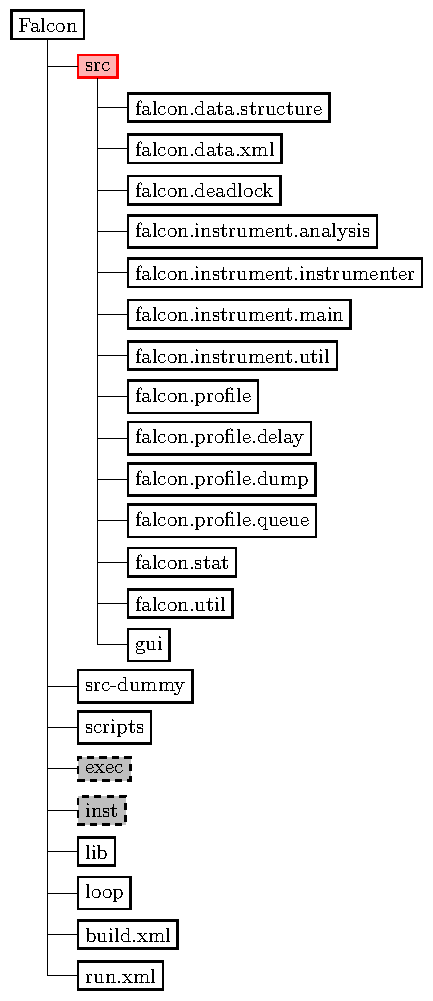
\includegraphics[width=.5\textwidth]{FileTree.pdf}
  \caption{Falcon文件组织框架}\label{pic:falconFrame}
\end{figure}
具体到src/目录里,falcon.data.structure里是Falcon中用到的数据结构。falcon.data.xml用来实现序列化和反序列化。falcon.deadlock 里的代码用于检测被测程序运行时是否死锁,如果死锁,execInfo里记录的运行结果将是Deadlock。falcon.instrument 里的代码用于实现插装。falcon.profile 里的代码主要是探针,用来插入到被测程序当中。
falcon.stat 里的代码用于统计结果,得到每一个模式的可疑度。falcon.util里的代码是Falcon中常用的数据类型。gui中的代码用于实现可视化。\par
scripts/下是Python脚本,用来自动化插装、运行多个被测程序。lib/下存放有Falcon中使用的类库。loop/有1.loop,10.loop,100.loop等文件,用来控制被测程序重复执行。build.xml和run.xml分别是使用ant进行编译和运行被测程序时的脚本。除了代码之外,还有inst和exec两个文件夹是运行Falcon过程中生成的,用来保存被测程序的插装结果和运行结果。\par
\subsection{被测程序的插装技术}
程序插装是指使被测试程序在保持原有逻辑完整性基础上在程序中插入一些探针,通过探针的执行并抛出程序的运行特征数据。基于这些特征数据分析,可以获得程序的控制流及数据流信息,进而得到逻辑覆盖等动态信息\cite{Instrument}。\par
实现插装时,Falcon使用Soot对被测程序进行静态的线程逃逸分析,从而确定一个变量是否被多个线程共享访问。如果一个变量是被多个线程访问,则插装该变量的读写操作,这样在程序运行时就可以得到访问共享变量的记录。如代码\ref{lst:inst}所示,对于一个Java语句``x = y + 1;'',在其前后分别进行插装探针,可以获得读变量y和写变量x的信息。
\begin{code}[language={[AspectJ]Java}, label=lst:inst, caption=插装程序读写操作示意]
  ...
  accessObj(method, Stmt(x=y+1), Var(y), read);
  x = y + 1;
  accessObj(method, Stmt(x=y+1), Var(x), write);
  ...
\end{code}
\subsubsection{线程逃逸分析}
在多线程程序当中,线程本地数据(thread local data)是指被一个线程拥有的数据。这里的``拥有''的意思是这些数据只能被这个线程访问\cite{threadlocal}。与之相对的是可以被多个线程访问的线程共享数据(thread shared data)。多个线程访问同一个数据可能会带来数据争用或死锁等问题。线程逃逸分析(thread escape analysis)的作用是监视所有对线程本地数据的访问,当检测到有另外一个线程尝试访问这个线程本地数据,即标记这个数据为逃逸(escaping)\cite{threadescape}。在Falcon中,首先需要通过线程逃逸分析判断一个变量是否被多个线程访问。
\subsubsection{Soot简介}
Soot是加拿大McGill大学Sable研究组开发的Java字节码分析和优化开源工具。它为字节码的分析、优化、反编译、注解等提供一个可扩展的框架\cite{jnuthesis2}。Soot作为字节码分析和转换工具,广泛地应用于编译器优化研究,程序分析等领域中。\par
Soot在Falcon工具中主要有三个作用。一是对被测程序进行静态的线程逃逸分析,用来确定一个变量是否被多个线程访问。在Soot的soot.jimple.toolkits.thread.ThreadLocalObjectsAnalysis包中提供了相应的API可以用来进行线程逃逸分
析\cite{halpert2008static}。二是使用Soot分析Java语句来判断线程对变量的访问是读还是写。三是使用Soot提供的API将探针插装到被测程序当中。
\subsubsection{插装的过程}\label{sec:InstProcess}
Soot的分析与变化是建立在其内部的中间表示法(Intermediate Representation,IR)上\cite{jnuthesis1}。 在Falcon中,使用的IR 是Jimple---Soot 中最核心的IR。在Soot里可以按照需要对Jimple进行分析、变换和优化,并生成相应.class文件。在Falcon进行插装时,需要运行falcon.instrument.main.Main.java。该类继承SceneTransformer类,重写了\texttt{internalTransformer()}方法,可以将探针插装到Jimple中间表示当中,最后用插装后的Jimple生成完成插装的.class文件。\\
\textbf{插装主方法}\par
为了便于Falcon判断进行插装的位置,首先需要对被测程序的\texttt{main()}方法进行修改成如下代码\ref{lst:uninstmain}所示。
\begin{lstlisting}[language={[AspectJ]Java}, label=lst:uninstmain, caption=未插装的被测程序主方法]
    public static void main(String[] args){
        runOneTest(args);
    }
\end{lstlisting}
即将原来的\texttt{main()}方法改名为\texttt{runOneTest()},然后重新写一个\texttt{main()}方法,并调用
\texttt{runOneTest()}方法。经过修改后,Falcon就可以按照下面代码\ref{lst:instmain1}所示完成对\texttt{main()}方法的插装。其中\texttt{startTestCase()}用来滑动窗口的初始化,\texttt{endTestCase()}用来返回被测程序的运行结果。\\
\begin{code}[language={[AspectJ]Java}, label=lst:instmain1, caption=插装后的被测程序主方法]
    public static void main(String[] args){
        startTestCase();
        runOneTest(args);
        finishTestCase();
    }
\end{code}\par
这里,还需要考虑的一个特殊情况就是带有静态类变量(带有static标识符)的主类。在Java语言中,静态变量在类创建的时候即在Java 虚拟机中完成分配内存、赋值等工作。这个时候如果仍然按照代码\ref{lst:instmain1}所示的方法进行插装,就无法对静态变量进行分析。在Jimple当中,静态变量、静态方法的初始化是在\texttt{<clinit>()}的方法内进行,因此需要将
\texttt{startTestCase()}插装到\texttt{<clinit>()}之前,如代码\ref{lst:instmain2}所示。
\begin{lstlisting}[language={[AspectJ]Java}, label=lst:instmain2, caption=插装后的带有静态变量的被测程序主方法]
    public static void main(String[] args){
        startTestCase();
        <clinit>()
        runOneTest(args);
        finishTestCase();
    }
\end{lstlisting}\par
插装主方法的过程中另外一个难点是在插装的\texttt{endTestCase()}中需要得到被测程序的运行结果作为参数传递给Falcon,但是被测程序的结果需要在运行结束后才能获得。这样就导致在Falcon运行时无法得到被测程序的结果,生成的execInfo.xml也存在错误。本文作者的解决方法是统一在插装\texttt{endTestCase()}时把被测程序的运行结果设置为通过,这样生成的execInfo.xml里记录的运行结果全部都是通过。然后使用Python脚本,读取被测程序运行日志文件里的结果来纠正execInfo.xml里的运行结果。\\
\textbf{插装方法}\par
对方法的插装在Falcon中是可选的操作。插装方法之后,可以获得被调用函数的信息。插装的过程是在每个方法的调用点和返回点插入探针,当程序运行时,每次调用一个方法,就会带出该方法的相关信息。\\
\textbf{插装变量}\par
在Falcon当中,对于变量的插装首先需要对Java中的语句进行分析,找出包含有对变量操作的语句。因此需要对Java字节码当中会出现所有的语句(Soot中Jimple里的Stmt类型)进行分情况讨论。虽然Jimple里语句共有15种,但除去调用语句、return语句、break 语句等大量不涉及变量读写操作的语句外,需要进行处理的语句只有4种,分别是If语句IfStmt、Switch语句TableSwitchStmt(对应于JVM里的tableswitch指令)和LookupSwitchStmt(对应于JVM里的lookupswitch指令)、赋值语句AssignStmt。代码片段如代码
\ref{lst:instStmt}所示。
\begin{lstlisting}[language={[AspectJ]Java}, label=lst:instStmt, caption=对不同的Stmt进行处理]
  ...
  if (StmtUtil.isReturnStmt(stmt)||stmt instanceof IdentityStmt||
      stmt instanceof EnterMonitorStmt||stmt instanceof NopStmt||
      stmt instanceof GotoStmt||stmt instanceof ExitMonitorStmt||
      stmt instanceof BreakpointStmt||stmt instanceof ThrowStmt){
      // do nothing
  } else if (stmt instanceof IfStmt) {
      //instrument if-stmt
      Value value = ((IfStmt) stmt).getCondition();
      instValue(stmt, value, true);
  } else if (stmt instanceof TableSwitchStmt){
      //instrument table switch
      Value value = ((TableSwitchStmt) stmt).getKey();
      instValue(stmt, value, true);
  } else if (stmt instanceof LookupSwitchStmt){
      //instrument lookup switch
      Value value = ((LookupSwitchStmt) stmt).getKey();
      instValue(stmt, value, true);
  } else if (stmt instanceof AssignStmt) {
      instAssignStmt((AssignStmt) stmt);
  }
  ...
\end{lstlisting}\par
找出了含有变量读写的语句之后,还需要要分析变量的读写操作和类型。对变量的读写操作可以通过语句的语义来进行判断。例如对于赋值语句“x=y”,可以知道赋值语句的右部,即变量y是读操作,而赋值语句的左部,即变量x是写操作。又如If语句和Switch语句里对条件的判断就是读操作。对变量的类型(基本数据类型或字段),可以使用Soot提供的API进行判断,在Falcon中,\texttt{instValue()}方法(如代码\ref{lst:instValue}所示)用来完成该任务。分析出变量的读写操作和类型之后,就可以将探针插装到程序中。\\
\begin{code}[language={[AspectJ]Java}, label=lst:instValue, caption=instValue()方法片段]
  private void instValue(Stmt stmt, Value value, boolean isRead){
    if (value instanceof StaticFieldRef) {
        instStaticFieldRef(stmt, value, isRead);
    } else if (value instanceof InstanceFieldRef) {
        instInstFieldRef(stmt, value, isRead);
    } else if (value instanceof InvokeExpr) {
        instInvokeExpr(stmt, value);
    } else if (value instanceof Local) {
        instLocal(stmt, value, isRead);
    } else if (value instanceof BinopExpr) {
        BinopExpr expr = (BinopExpr) value;
        instValue(stmt, expr.getOp1(), true);
        instValue(stmt, expr.getOp2(), true);
    } else if (value instanceof UnopExpr) {
        UnopExpr expr = (UnopExpr) value;
        instValue(stmt, expr.getOp(), true);
    } else {
        // print no-instrumented value
        ...
    }
  }
\end{code}\par
关于插装被测程序,被分析的原有代码缺少了对If语句和Switch语句这两个情况的考虑。原有代码也没有处理带有静态类变量的主类。本文作者补充了代码从而解决了上述两个不足。
\subsection{串行化为XML和反序列化为对象}
在Falcon运行的过程中,需要将运行中间的插装信息、被测程序的运行结果和输出结果进行序列化成XML文件进行保存。在分析、统计的过程中,也需要将XML文件里的结果反序列化成内存中的对象进行处理。
\subsubsection{XStream简介}
XStream是由codehaus项目组开发的Java类库,用来将对象序列化成XML(JSON)或反序列化为对象\cite{xstream}。使用XStream不用任何映射就能实现多数Java对象的序列化。在生成的XML中对象名变成了元素名,类中的字符串组成了XML中的元素内容。使用XStream序列化的类不需要实现Serializable接口。XStream是一种序列化工具而不是数据绑定工具,就是说不能从XML或者XML Schema Definition (XSD) 文件生成类。和其他序列化工具相比,XStream 有三个突出的特点:
\begin{enumerate}
  \item XStream不关心序列化/逆序列化的类的字段的可见性。
  \item 序列化/逆序列化类的字段不需要 getter 和 setter 方法。
  \item 序列化/逆序列化的类不需要有默认构造函数。
  \item 不需要修改类,使用 XStream 就能直接序列化/逆序列化任何第三方类\cite{xstream_ibm}。
\end{enumerate}
\subsubsection{串行化和反序列化的过程}
在falcon.data.structure包中共有三个类用来保存程序运行的中间信息,分别是保存插装信息的InstInfo,被测程序运行信息的ExecInfo和Falcon结果的SummaryInfo。这三个类需要实现序列化和反序列化。在falcon.data.xml包中,UML类图如图
\ref{pic:FalconXML}所示。
\begin{figure}[!ht]
  \centering
  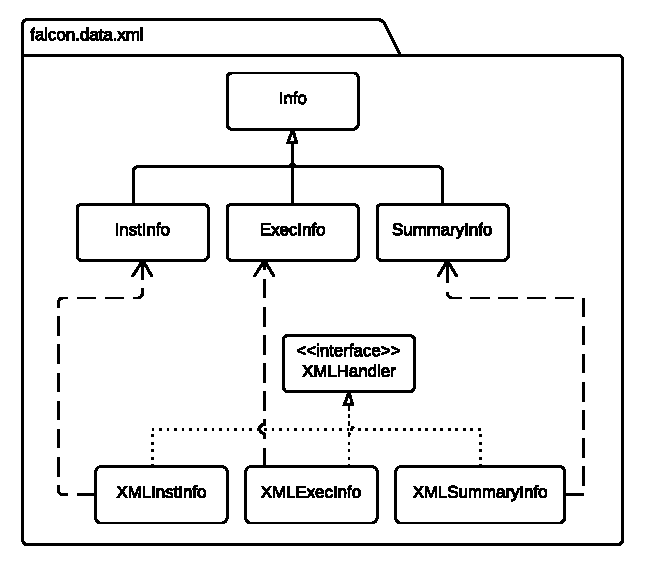
\includegraphics[width=.8\textwidth]{FalconXML.pdf}\\
  \caption{falcon.data.xml包UML类图}\label{pic:FalconXML}
\end{figure}
首先创建XMLHandler接口,包含有\texttt{Serialize(Info, path)}和\texttt{deSerialize(path)}两个方法。再分别创建XMLInstInfo、XMLExecInfo和XMLSummaryInfo 三个类来实现XMLHandler接口。\par
InstInfo类包括被调用的方法列表和程序中出现的变量构成的列表。经过序列化之后生成的instInfo.xml的片段如代码
\ref{lst:instxml}所示,XML元素的解释见表\ref{tab:instXMLele}。\\
\begin{code}[language=XML, label=lst:instxml, caption=instInfo.xml片段]
<methodInfo>
 <mid>4</mid>
 <msig>&lt;contest.account.Account: void transfer(...)&gt;</msig>
</methodInfo>
<variableInfo>
 <vid>6</vid>
 <vtype>WF</vtype>
 <vsig>this.&lt;contest.account.Account:double amount&gt;</vsig>
 <vfile>Account.java</vfile>
 <vline>24</vline>
</variableInfo>
\end{code}
\begin{table}[!ht]
    \centering
    \zihao{4}
    \caption{instInfo.xml元素介绍}\label{tab:instXMLele}
    \begin{tabular}{|l|l|}
      \hline
       XML文档元素 & 解释\\\hline
       <mid>4</mid> & 方法的编号为4\\\hline
       <msig>...</msig> & 方法的签名\\\hline
       <vid>6</vid> & 变量的编号是6\\\hline
       <vtype>WF</vtype> & 变量的操作类型是写类属性\\\hline
       <vsig>...</vsig> & 变量的签名\\\hline
       <vfile>Account.java</vfile> & 变量在Account.java文件中\\\hline
       <vline>24</vline> & 变量出现在第24行\\\hline
    \end{tabular}
\end{table}\par
ExecInfo类包含有该次程序运行的结果和出现的数据访问模式。经过序列化之后生成的execInfo.xml。SummaryInfo类包含有多次运行结果的统计信息和各个数据访问模式的信息、可疑度。其中,顺序破坏和原子性破坏这两种数据访问模式是最主要的信息。经过序列化后,这两部分信息会如代码\ref{lst:execxml}所示保存成XML文档,其中XML元素的解释见表\ref{tab:execXMLele}。\\
\begin{code}[language=XML, label=lst:execxml, caption=execInfo.xml片段]
<order>
    <pass>9</pass>
    <fail>1</fail>
    <susp>10</susp>
    <stack1></stack1>
    <stack2></stack2>
    <var1>6</var1>
    <var2>8</var2>
</order>
<atomicity>
    <pass>0</pass>
    <fail>1</fail>
    <susp>100</susp>
    <stack1></stack1>
    <stack2></stack2>
    <var1>4</var1>
    <var2>2</var2>
    <stack3></stack3>
    <var3>27</var3>
</atomicity>
\end{code}
\begin{table}[!ht]
    \centering
    \zihao{4}
    \caption{数据访问模式序列化为XML}\label{tab:execXMLele}
    \begin{tabular}{|l|l|}
      \hline
      XML文档元素 & 解释\\\hline
       <pass>9</pass> & 被测程序执行了10次,其中9次得到正确结果\\\hline
       <fail>1</fail> & 被测程序有一次运行结果错误\\\hline
       <susp>10</susp> & 可疑度是10\%\\\hline
       <var1>6</var1> & 模式的第一个操作的变量编号是6\\\hline
       <stack1></stack1> & 方法调用序列\\\hline
    \end{tabular}
\end{table}
\subsection{改进}
由于被分析的源码并不完整,需要对代码进行补充才能够运行。另外,本文以Martin Fowler的《重构——改善既有代码的设计》一书为指导,对源代码的部分实现过程进行了重构。虽然重构的操作比较琐碎,但是提高了代码的可读性,一些代码做到了复用。
\subsubsection{对源代码的补充}
被分析的源代码由于不完整,因此不能够对\texttt{startTestCase()} 和\texttt{endTestCase()}进行插装。缺少的这一部分代码涉及到了滑动窗口的初始化和返回被测程序运行结果等关键步骤,所以必须补充完整才能使Falcon运行。本文作者补充了这一部分的代码,使Falcon可以运行。此外,本文作者对Falcon 原有算法的完善主要包括两点:
\begin{enumerate}
  \item 增加了对If语句和Switch语句的分析;
  \item 增加了对含静态变量的类的处理。
\end{enumerate}
关于以上两点的具体实现,本文作者所做的工作在\ref{sec:InstProcess}中已做了具体介绍和解释。
\subsubsection{对Falcon的重构}
本次毕业设计中对原有代码的重构包括以下几点:\\
1. 封装字段\\
falcon/data/structure中部分类中public字段改为private,并且加入相应的访问函数。\\
2. 重构部分方法
\begin{itemize}
  \item 提炼函数,将过长的代码段放入独立的函数中,如添加ExecInfo类, SummaryInfo类中\texttt{print()}方法等;
  \item 以直接访问类属性取代方法调用,修改InstMethod类和InstVariable类的toString方法,减少方法调用次数,提高效率。
\end{itemize}
3. 使用Enum类型
\begin{itemize}
  \item 添加ExecuteResult枚举类,替换之前使用int类型表示运行结果;
  \item 重写EventType枚举类,添加\texttt{toString()}方法,删去\texttt{getTypeString()} 方法。
\end{itemize}
4.提炼接口\\
将用于序列化和反序列化的\texttt{Serialize()}和\texttt{deSerialize()}提炼到一个独立的接口中。\\
5.提炼超类\\
将ExecInfo、InstInfo和SummaryInfo三个类中相同的属性和方法移至超类Info中。\\
6. 修改部分代码,使满足编程规范。
\subsection{运行环境与配置}
\subsubsection{运行环境}
\noindent 硬件
\begin{itemize}
  \item CPU:Intel Core 2 Duo T6500, 2.1GHz
  \item 内存:2G
\end{itemize}
软件
\begin{itemize}
  \item Java运行环境:Java SE 1.7
  \item Python运行环境:Python3.3
  \item 开发环境:Eclipse 4.2
  \item 构建工具:Apache Ant 1.8.4
  \item 基准程序: The ConTest Benchmark Suite
  \item Soot 2.4.0\footnote{目前Soot的最新版本是2.5.0,但是使用该版本有兼容性问题。}
\end{itemize}\par
Apache Ant是一个将Java编译、测试、部署等步骤联系在一起加以自动化的一个工具,脚本格式为XML。Ant和C语言使用的make脚本一样,可以用于自动化调用程序完成项目的编译,打包,测试等。Python是一门面向对象的解释型编程语言。在Falcon当中,使用Python 脚本用来调用Ant的build文件,便于自动化运行多个被测程序。The ConTest Benchmark Suite由一组包含有并发错误的Java 多线程小程序(代码行均小于1000行)组成的基准程序,可以用来检验多线程测试工具的有效性\cite{eytani2007towards}。 ConTest Benchmark里的程序都给出了具体的场景,即预期的输出结果,这样便于判断程序的实际输出结果是否正确。程序中的错误在文档里都进行了详细的分析和说明,这样便于和错误定位工具得到的结果进行比对,从而可以检测工具的有效性。
\subsubsection{配置过程}
\begin{enumerate}
  \item 安装Eclipse插件
  \begin{itemize}
    \item Python插件PyDev\footnote{http://pydev.org/download.html}
  \end{itemize}
  \item 创建工作目录(Falcon\_Root)
  \item 创建子目录
  \begin{itemize}
    \item Falcon\_Root/falcon,用来存放Falcon代码
    \item Falcon\_Root/subjects,用来存放基准程序
    \item Falcon\_Root/library,用来存放类库
  \end{itemize}
  \item 添加需要的类库至Falcon\_Root/library
  \begin{itemize}
    \item sootclasses.jar
    \item jasminclasses.jar
    \item java\_cup.jar
    \item polyglot.jar\footnote{以上四个jar包均可以在http://www.sable.mcgill.ca/soot/soot\_download.html下载。}
    \item xpp3\_min.jar\footnote{http://mvnrepository.com/artifact/xpp3/xpp3\_min}
    \item xstream.jar\footnote{http://xstream.codehaus.org/download.html}
  \end{itemize}
  \item 导入项目代码,配置类库路径
\end{enumerate}
\subsubsection{运行}
Falcon运行的流程如图\ref{pic:FlowDiagram}所示。
\begin{figure}[!ht]
  \centering
  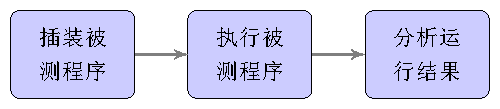
\includegraphics[width=.8\textwidth]{FlowDiagram.pdf}\\
  \caption{Falcon运行流程图}\label{pic:FlowDiagram}
\end{figure}\par
在Eclipse上运行,具体包括一下几个步骤:\\
1.编译\\
编译Falcon和Benchmark。在Eclipse中,可以直接右键build.xml选择执行ant。\\
2.插装\\
运行inst.py,调用build.xml中的inst任务进行插装。在安装过PyDev的Eclipse中,可以直接运行python脚本。\\
3.运行\\
运行exec.py,调用run.xml运行被测程序。\\
4.纠正运行结果\\
运行result.py,读取日志文件纠正execInfo.xml中错误的运行结果。\\
5.输出排序结果\\
运行output.py,调用run.xml得到统计结果。
\subsection{运行结果}
\noindent\textbf{插装结果}\par
第一步插装之后,Falcon会生成记录静态分析被测程序过程的日志文件和保存有插装结果的instInfo.xml,同时,还会得到经过插装的.class文件。\\
\textbf{运行结果}\par
第二部运行经过插装的被测程序(第一步生成的经过插装的.class文件),每运行一次被测程序,会生成带有运行结果的日志文件(.log)和保存有每一个数据访问模式的execInfo.xml。\\
\textbf{输出结果}\par
最后一步之后,Falcon会生成两个文件来保存结果,分别是序列化后的summaryInfo.xml和显示结果的rank.txt。其中rank.txt的输出结果如下所示。\\
~\\
\fbox{
\begin{minipage}{.95\textwidth}
\zihao{5}
--------------------------------------------------------\\
		Result\\
--------------------------------------------------------\\
Total Pass: 3\\
Total Fail: 7\\
Total Deadlock: 0\\
--------------------------------------------------------\\
		printing order violation\\
| rank | pass | fail | deadlock | access1 | access2 | score |\\
--------------------------------------------------------\\
| 1 | 3 | 7 | 0 | WF @Account.java:25 | WF @Account.java:26 | 70.0\% |\\
| 2 | 0 | 3 | 0 | RF @Account.java:31 | WF @Account.java:21 | 42.0\% |\\
| 3 | 0 | 3 | 0 | WF @Account.java:26 | RF @Main.java:73 | 42.0\% |\\
\ldots\\
--------------------------------------------------------\\
		printing atomicity violation\\
| rank | pass | fail | deadlock | access1 | access2 | access3 | score |\\
--------------------------------------------------------\\
| 1 | 3 | 7 | 0 | RF @Account.java:31 | WF @Account.java:25 | RF @Main.java:73 | 70.0\% |\\
| 2 | 3 | 7 | 0 | RF @Account.java:31 | WF @Account.java:26 | RF @Main.java:73 | 70.0\% |\\
| 3 | 0 | 4 | 0 | RF @Account.java:26 | WF @Account.java:25 | WF @Account.java:26 | 57.0\% |\\
| 4 | 1 | 4 | 0 | WF @Account.java:21 | WF @Account.java:26 | WF @Account.java:25 | 50.0\% |\\
| 5 | 0 | 3 | 0 | RF @Account.java:31 | WF @Account.java:25 | RF @Main.java:71 | 42.0\% |\\
| 6 | 0 | 3 | 0 | RF @Account.java:31 | WF @Account.java:26 | RF @Main.java:71 | 42.0\% |\\
\ldots\\
\end{minipage}
}\\
~\par
示例的程序是The ConTest Benchmark Suite中的一个小程序。经过插装后共运行了10遍。首先Result显示了这10次运行,一共有3次通过,剩下7次得到的结果都与预期不符,没有出现死锁。接着显示的是按照可疑度由高到低排列的顺序破坏数据访问模式。其中,排名第1 的模式是$W_1-W_2$型的顺序破坏。变量所在的位置分别是Account.java的第25行和Account.java的第26行。在10次运行中,有3次结果正确,7 次结果错误。按照公式\ref{Jaccard}可以计算出可疑度是70\%。顺序破坏数据访问模式过后,显示的是按照可疑度由高到低排列的原子性破坏数据访问模式,输出信息的具体含义与顺序破坏的相同。

    \section{Falcon工具的可视化}
\subsection{可视化的目标}
原始版的Falcon工具虽然可以具体定位到每一个数据访问模式的变量名和所在的语句,但由于结果只能以纯文字的格式显示,仍然不便于程序员迅速发现和定位错误。所以本文作者希望能够通过高亮显示的方式来突出包含错误模式的语句。同时希望将选择被测程序、插装、运行被测程序等一系列操作统一到一个图形化界面的工具里。
\subsection{可视化的实现}
\subsubsection{MVC设计模式}
MVC模式(Model-View-Controller)是软件工程中的一种软件架构模式。MVC是以模型(Model)、视图(View)和控制器(Controller)三个单词的首字母缩写命名。使用MVC模式可以减少代码之间的耦合。MVC模式的三个模块相互独立,改变其中一个不会影响其他两个,从而提高了应用程序的灵活性和可配置性。\par
模型用来封装应用程序的业务逻辑和基础数据。模型对外提供接口,可以被控制器和视图调用。视图是应用程序与用户的接口,作用是负责显示,即表达逻辑的内容。视图是模型的外观,可以访问模型的数据,但不能改变这些数据。视图只需要知道模型提供的接口,而不需要了解模型的内部逻辑。控制器是模型和视图之间的桥梁。控制器的作用是接受视图请求,并做出反应,执行相应的控制流,或者把响应结果返回到视图\cite{LiMVC}。\par
在Falcon可视化工具的实现过程中使用了MVC设计模式,这一部分的UML图如图\ref{pic:MVCUML}所示。
\begin{figure}[!ht]
  \centering
  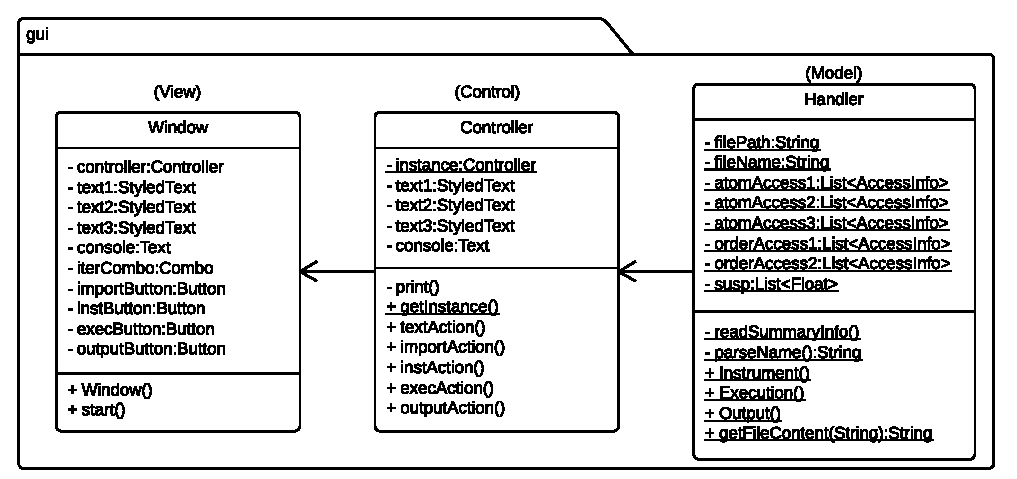
\includegraphics[width=\textwidth]{MVCUML.pdf}\\
  \caption{MVC设计模式的UML类图}\label{pic:MVCUML}
\end{figure}
\subsubsection{SWT框架}
SWT(Standard Widget Toolkit,标准部件工具包)是在Java平台下的一个图形化部件工具包。SWT最初由IBM公司主导开发,现在作为Eclipse集成开发环境的一部分由Eclipse基金会维护\cite{swt_wiki}。\par
和Java AWT、Java Swing等其它相比,SWT主要有以下优势:
\begin{enumerate}
  \item 界面与本地操作系统对应;
  \item 简单实用的API可以是开发人员快速上手;
  \item SWT应用程序运行速度快\cite{SWT}。
\end{enumerate}\par
在Falcon的可视化工具中,如何使含有错误的代码高亮显示是一个难点。在SWT中,提供了StyledText部件可以用来显示带有格式的文本,实现诸如加粗、背景色等显示效果。在窗口中添加StyledText对象,并调用\texttt{addLineBackgroundListener()}方法,实现LineBackgroundListener接口中的\texttt{lineGetBackground()}方法,即设定需要高亮显示的行数\textit{line}和背景的样式。当StyledText 对象中加入了文字之后,就可以触发LineBackgroundEvent,LineBackgroundListener监听到事件后,就把第\textit{line} 行按照之前的设置高亮显示出来。
\subsection{可视化的效果}
Falcon的可视化工具效果如截图\ref{Screen}所示。
\begin{figure}[!ht]
  \centering
  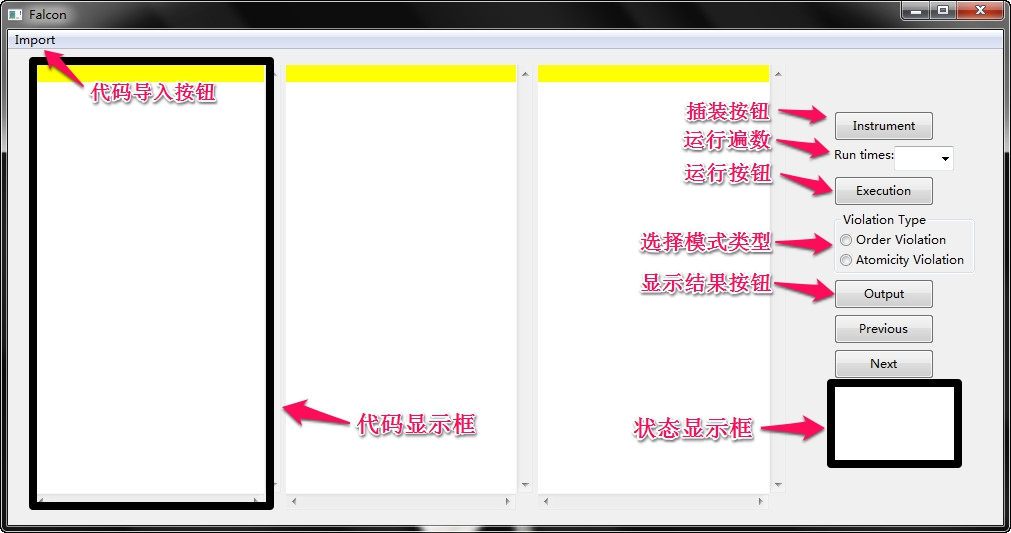
\includegraphics[width=.8\textwidth]{Screen.jpg}\\
  \caption{Falcon的可视化工具}\label{Screen}
\end{figure}
在使用时,首先需要导入被测程序。点击菜单栏上的Import按钮,选择被测程序中包含有主方法的类。如图\ref{ChooseFile}所示。
\begin{figure}[!ht]
  \centering
  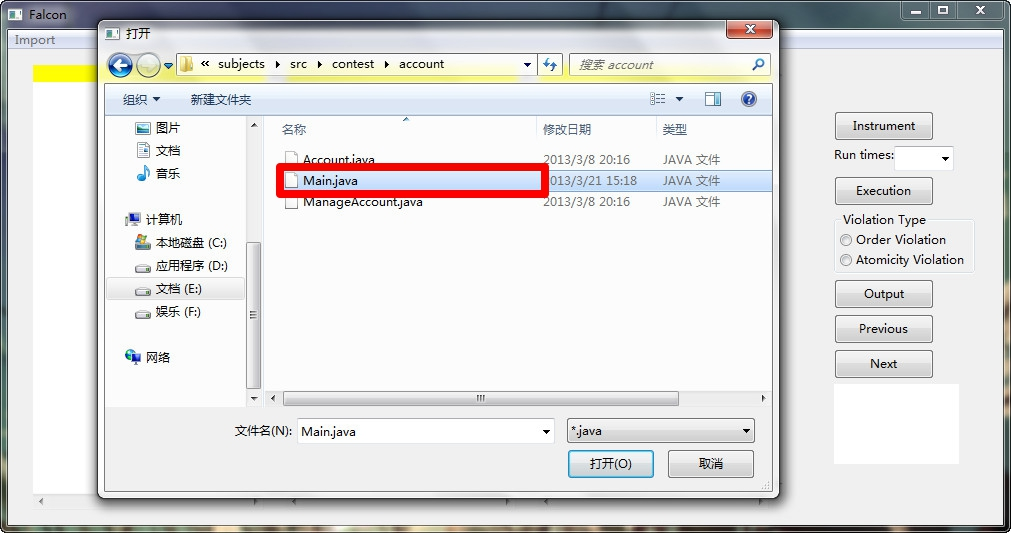
\includegraphics[width=.8\textwidth]{ChooseFile.jpg}\\
  \caption{选择被测程序中包含有主方法的类}\label{ChooseFile}
\end{figure}
点击Instrument按钮可以进行插装。在Run Times里可以选择被测程序执行的次数,然后点击Execution按钮可以运行被测程序。点击Output按钮之后,文本框中会出现被测程序的代码。包含有错误的访问模式所在的代码行被黄色高亮显示。在右下角的显示框内,会显示这个访问模式的具体信息,包括可疑度,模式类型,变量名等。
\begin{figure}[!ht]
  \centering
  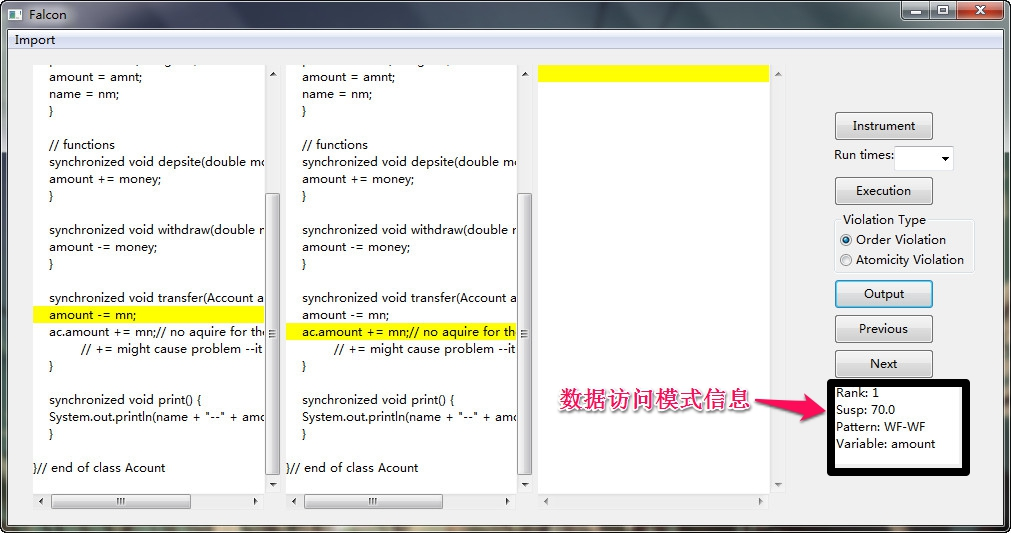
\includegraphics[width=.8\textwidth]{order.jpg}\\
  \caption{顺序性破坏显示效果}
\end{figure}
点击Next按钮则可以显示后一个错误的模式,点击Previous按钮可以显示前一个错误的模式。
\begin{figure}[!ht]
  \centering
  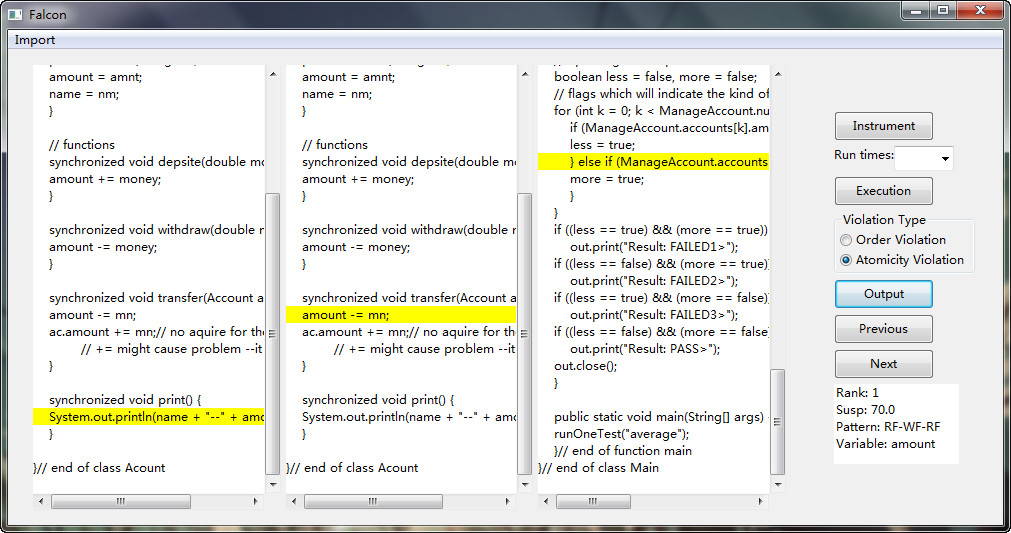
\includegraphics[width=.8\textwidth]{atom.jpg}\\
  \caption{原子性破坏显示效果}
\end{figure}
\subsection{与CORE的对比}
在Sangmin Park提出了Falcon的方法之后,乔治亚理工学院的两个研究生,Deepal Jayasinghe和Pengcheng Xiong,也尝试将Falcon扩展成为可视化工具。他们最终开发出了名为CORE的可视化并发错误定位工具\cite{CORE}。\par
CORE可以提供两个层次的视图来显示结果。如图\ref{pic:core}所示,低层次的视图用来显示数据访问模式中变量和方法的详细信息。高层次的视图用来显示模式的的可疑度等统计信息。此外,CORE提供了更为丰富的信息,包括插装信息、方法调用序列等。
\begin{figure}[!ht]
  \centering
  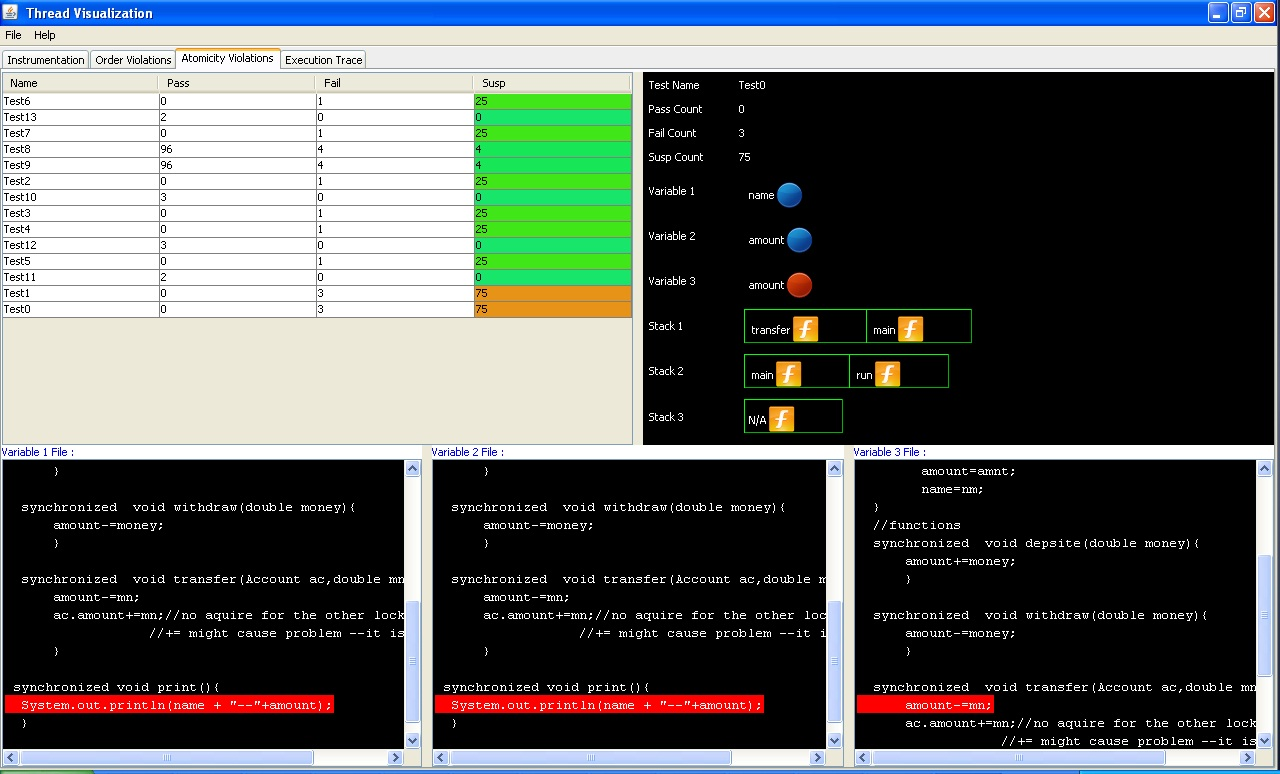
\includegraphics[width=.8\textwidth]{CORE.jpg}\\
  \caption{CORE的显示效果}\label{pic:core}
\end{figure}
与CORE相比,本文中的可视化工具有如下特点:
\begin{enumerate}
  \item 界面更加简洁;
  \item 操作更加简单;
  \item 将插装、运行被测程序这两个步骤集中到可视化工具当中。
\end{enumerate}

    \section{总结与展望}
本论文主要完成的工作包括以下几个方面:
\begin{enumerate}
  \item 分析了多线程程序错误定位工具的价值;
  \item 通过实例叙述了Falcon算法的过程;
  \item 详细描述了Falcon原始版本的实现和本文作者重构过程;
  \item Falcon的配置和运行;
  \item 详细描述了Falcon可视化工具实现的过程和效果。
\end{enumerate}\par
本文通过上述工作,详细地描述了Falcon算法的原理,并且通过对实例的说明,直观地展示了Falcon运行过程中重要的步骤。对Falcon实现过程中的几个重要部分和可视化的实现过程进行了细致的介绍。此外,在论文里还详细地列出了如何配置、运行Falcon。\par
最后,虽然已经做出了一个具有可视化功能的原型,但是仍然有可以改进的地方。例如,界面还不美观;只能显示单个访问模式的信息,不能像CORE一样显示一个被测程序总体的运行结果。此外,Falcon实现之后只在The ConTest Benchmark上进行了测试并取得了很好的效果,今后还需要使用更多的程序来验证Falcon的健壮性和有效性。这些不足需要在今后的学习中加以完善。

%%----------------- 附件 ----------------- %%
    \begin{center}
  \zihao{-2}\textbf{\songti 致谢}
\end{center}\par
\zihao{4}\songti
在此,我要感谢本篇论文的指导教师孙玉霞老师。感谢她对我的悉心指导,并且为我毕业论文的撰写指明方向。同时也要感谢大学四年里教过我的所有任课老师,我能够完成毕业论文离不开他们的辛勤栽培。\par
感谢McGill大学的Sable实验室、Codehaus项目组、PyDev项目组以及Eclipse基金会,正是他们的开源项目为本次毕业论文的实验部分无偿提供了必需的工具。还要感谢TUG和CTeX社区,他们为本次毕业论文的撰写和排版提供了优秀的工具。\par
......\par
谨把本文献给我最敬爱的父亲、母亲以及所有关心我、帮助我的人!\par
%END

    \bibliographystyle{GBT7714-2005NLang}
    \bibliography{reference}
\end{document}
